\documentclass[../main.tex]{subfiles}

\begin{document}

For a while, we even considered splitting the adjuster into a separate project. But in case of a split, we would need to split the rest of the project into a core (containing all the common abstractions) and everything else (which would use the core). Adjuster would in that case use a core as its dependency. This separation would either mean 3 separate projects (which would lead from our considerations to more drawbacks than benefits) or a project with 2 modules, and a single-module Adjuster project. In the end, separating the whole project into 3 modules (adjuster, core, and everything else) seemed like the most suitable solution, which was chosen. These 3 modules, together with their inter-module dependencies, are shown in Figure \ref{fig:reqour-modules}. All 3 modules have separate YAML configurations\footnote{\url{https://quarkus.io/guides/config-yaml}} mapped to Java objects\footnote{\url{https://quarkus.io/guides/config-mappings}}.

\begin{figure}
  \begin{center}
    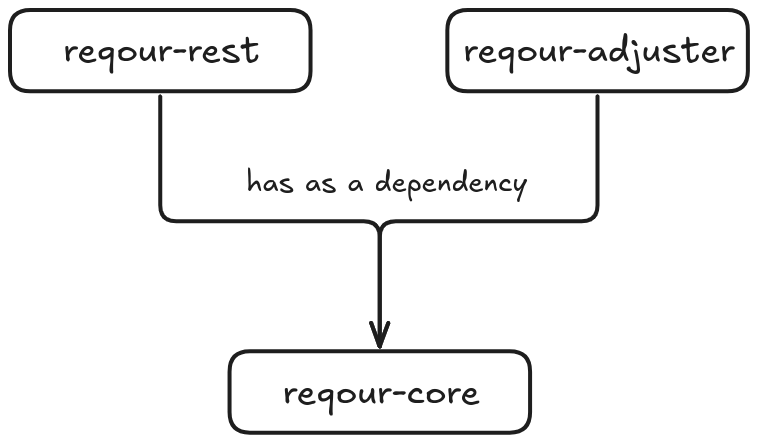
\includegraphics[width=0.7\textwidth]{images/reqour-modules.png}
  \end{center}
  \caption{Overview of Reqour implementation}
  \label{fig:reqour-modules}
\end{figure}

\end{document}
